
\documentclass[12pt]{article}
\usepackage[english]{babel}
\usepackage[utf8x]{inputenc}
\usepackage{amsmath}
\usepackage{graphicx}
\graphicspath{ {scrn/} }
\usepackage[colorinlistoftodos]{todonotes}

\begin{document}

\begin{titlepage}

\newcommand{\HRule}{\rule{\linewidth}{0.5mm}} % Defines a new command for the horizontal lines, change thickness here

\center % Center everything on the page
 
%----------------------------------------------------------------------------------------
%	HEADING SECTIONS
%----------------------------------------------------------------------------------------

\textsc{\Large UNIVERSITATEA TEHNICĂ A MOLDOVEI}\\[1cm] % Second title
\textsc{\Large Facultatea „Calculatoare, Informatică şi Microelectronică”}\\[0.5cm] % Third title
\textsc{\large Specialitatea : Tehnologii informationale}\\[0.5cm] % Minor heading 

\textsc{\large Disciplina : Medii interactive de dezvoltare a produselor soft}\\[1cm] % Minor heading 
\large Lucrarea de laborator nr.4\\[1cm]
%----------------------------------------------------------------------------------------
%	TITLE SECTION
%----------------------------------------------------------------------------------------

\HRule \\[0.4cm]
{ \huge \bfseries Dezvoltarea unei aplicatii mobile}\\[0.2cm] % Title of the document
\HRule \\[2cm]
 
%----------------------------------------------------------------------------------------
%	AUTHOR SECTION
%----------------------------------------------------------------------------------------

\begin{minipage}{0.4\textwidth}
\begin{flushleft} \large
\emph{A efectuat:}\\
\emph{}\\
\emph{A verificat:}\\
\end{flushleft}
\end{minipage}
~
\begin{minipage}{0.4\textwidth}
\begin{flushright} \large
st. gr. TI-141 \\
\textsc{Levcenco Elena}\\ % Student's Name
\textsc{ Cojanu Irina} % Teacher's Name
\end{flushright}
\end{minipage}\\[3cm]

%----------------------------------------------------------------------------------------
%	DATE SECTION
%----------------------------------------------------------------------------------------

{\large \today}\\[2cm] % Date, change the \today to a set date if you want to be precise

%----------------------------------------------------------------------------------------

\vfill % Fill the rest of the page with whitespace

\end{titlepage}
\section{Scopul lucrarii:}
Cunoasterea unui IDE care permite crearea aplicatiilor mobile si studierea functiilor de baza unui SDK.Compilarea si crearea unei aplicatii finale(apk) 
\section{Obiective:}
\begin{itemize}
\item Cunostinte de baza privina arhitectura unei aplicatii mobile
\item Cunostinte de baza ale platformei SDK
\end{itemize}
\section{Laboratory Requirements}
\begin{itemize}
\item Aplicatia trebuie sa fie dezvoltata si testata cu orice SDK ce include Emulator.
\item Testarea aplicatiei pe un device real
\item Aplicatia trebuie sa suporte device-urile cu diferite rezolutii
\item Realizeaza o aplicatie care va implimenta tehnica Pomodoro SAU
\item O alta aplicatie sofisticata la alegere
\end{itemize}


\label{sec:examples}

\section{Analiza lucrarii:}
IDE-ul:Android studio\\
Sistemul informaţional ”Official Alert” are componente pe platforma mobile, aplicaţia Android.Interfaţa aplicaţiilor este identică ca şi funcţionalul pe pagina web. Pentru prima dată cînd se lansează aplicaţia utilizatorul are pe prima pagină vede ultimele noutăţi de la fiecare sursă guvernamentală de informaţie. Pe această pagină vedem denumirea noutăților, o mică descriere si un buton de reînprospătare a noutăților.În aplicaţie avem disponibil un meniu care ne ghidează spre setările aplicaţiei, totodată nu avem logarea prezenta în aplicaţie precum utilizăm că identificator al utilizatorului însuşi identificatorul dispozitivului. Meniul lateral care are patru opţiuni:
\begin{itemize}
\item marchează că citit;
\item despre noi;
\item setări;
\item push-notificare.
\end{itemize}	
	Următoarea pagina este pagina unde putem gestiona sursele la care sîntem abonaţi că utilizator.\\
    Ionic este un sistem complet SDK open-source pentru dezvoltarea de aplicații mobile hibride.Aplicațiile pot fi construite cu aceste tehnologii Web și apoi distribuite prin magazinele de aplicații native care urmează să fie instalat pe dispozitive de pârghie Cordova.
\\
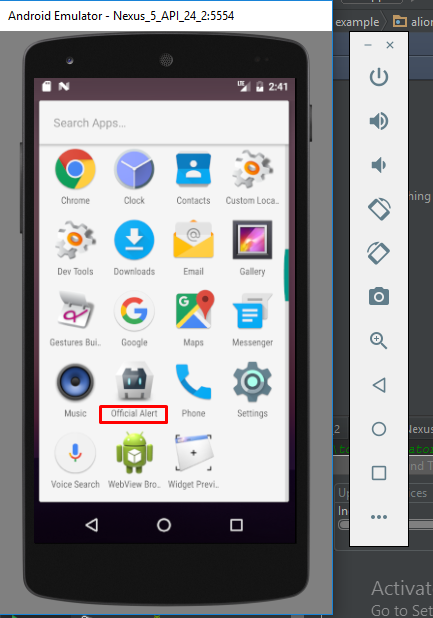
\includegraphics{1.png}\\
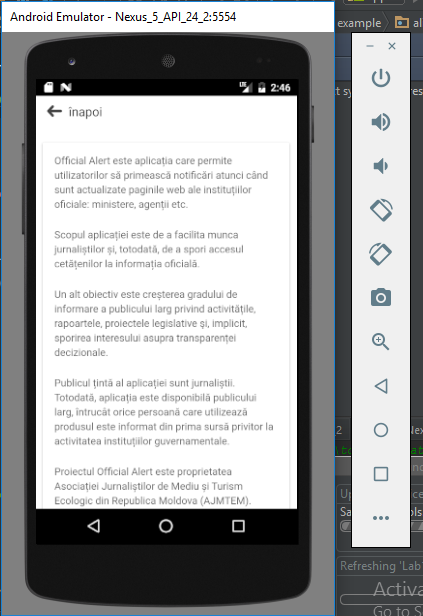
\includegraphics{2.png}\\
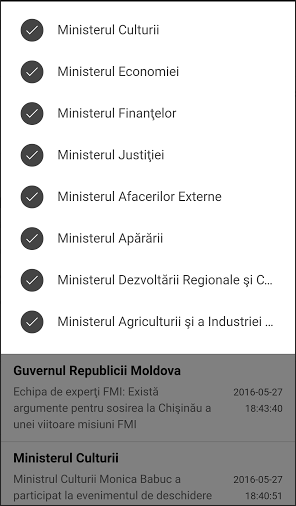
\includegraphics{3.png}\\
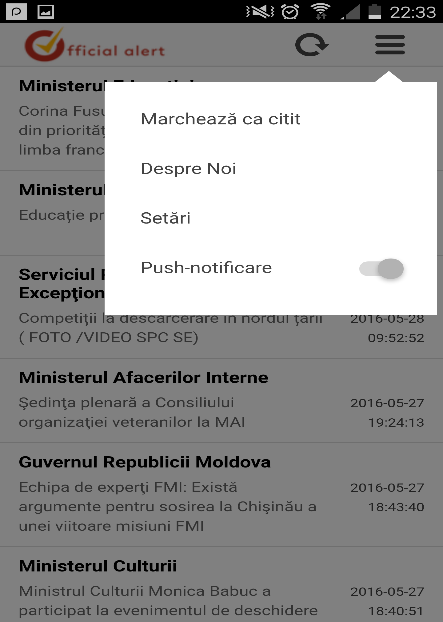
\includegraphics{4.png}
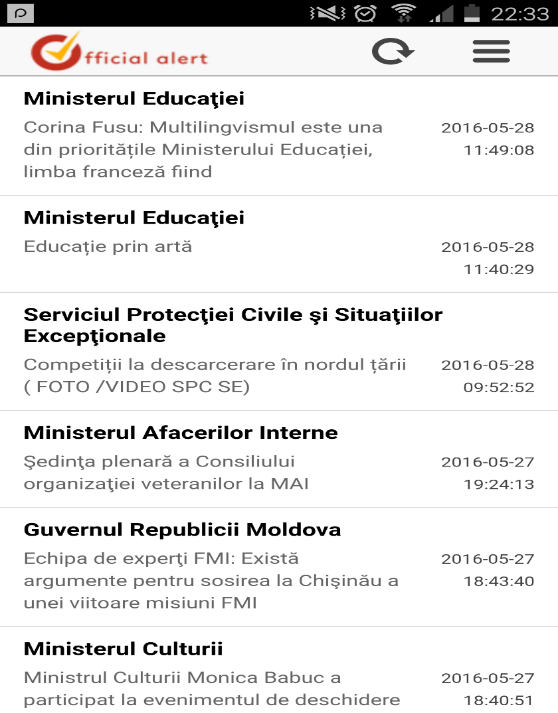
\includegraphics{5.png}\\

\section*{Concluzia}
Atunci cand avem nevoie sa dezvoltam in acelasi timp o aplicatie pentru Android si una pentru iOS, Ionic este solutia la care apelam de cele mai multe ori. Clasele sale de tip Bootstrap ne permit sa dezvoltam rapid interfete frumoase.Nu este doar mai rapid de dezvoltat astfel, dar partea de maintenance este mult simplificata, la care se adauga beneficiile suportului in timp real din partea Ionic, volumul mare si in continua crestere de resurse online si update-urile rapide pentru a tine pasul cu noile versiuni ale tehnologiilor conexe, ca Angular 2.0.Ionic asigura toate functionalitatile care se gasesc in SDK-urile mobile native. Permite dezvoltarea de aplicatii, customizarea lor pentru Android si iOS si lansarea prin Cordova. Ionic include componente mobile, tipografie, paradigme interactive si o tema de baza extensibila.In afara de SDK, Ionic ofera si serviciile prin care programatorii pot crea feature-uri, precum notificari push, testare A/B, analiza, lansari de cod si build-uri automatizate.
\end{document}